\documentclass[sigconf,nonacm]{acmart}

\AtBeginDocument{%
  \providecommand\BibTeX{{%
    Bib\TeX}}}

% --- TikZ Graphics Configuration for Architecture Diagrams ---
\usepackage{tikz}
\usetikzlibrary{arrows.meta, positioning, shapes.geometric, calc}
\setlength{\emergencystretch}{3em}

\setcopyright{none}
\copyrightyear{2026}
\acmYear{2026}

\title{Context Sphere: Topology-Aware Context Orchestration for Cost-Efficient LLM Repository Repair}

\author{Yuwen Zhang\footnote{PhD candidate, School of Aerospace, Mechanical and Mechatronic Engineering}}
\affiliation{%
  \institution{The University of Sydney}
  \city{Sydney}
  \state{NSW}
  \postcode{2006}
  \country{Australia}}

\begin{abstract}
Autonomous software-engineering agents built on LLMs show promise across repository navigation, repair, refactoring, and review, but they still struggle with context management in large repositories. Static retrieval often causes either context dilution or information amputation by breaking structural dependencies.

We present \textbf{Context Sphere}, a topology-aware framework that combines neural centroid selection with deterministic AST-based neighborhood expansion, then routes the bounded context through an adversarial Product Manager--Worker--Reviewer state machine.

On a 100-case evaluation using a local \texttt{PASS\_TO\_PASS} verification harness over pure-Python SWE-bench Verified instances, Context Sphere achieved 41 successful local repair passes, compared with 36 passes for a dense vector baseline at roughly \$0.08 per issue. A naive Hybrid retriever reached 39 passes, revealing that dense-first merging can displace structurally important dependency files. A preliminary 10-case projection study shows that persona-conditioned routing with a Top-\(K\) safety floor can preserve 9/10 known successes while cutting input tokens by 71.5\% and estimated cost by 58.4\%.

We provide an artifact repository to support reproducibility and position this work as a foundation for future official SWE-bench \texttt{FAIL\_TO\_PASS} evaluation.

\end{abstract}

\begin{CCSXML}
<ccs2012>
 <concept>
  <concept_id>10011007.10011006.10011050</concept_id>
  <concept_desc>Software and its engineering~Software testing and debugging</concept_desc>
  <concept_significance>300</concept_significance>
 </concept>
 <concept>
  <concept_id>10010147.10010257.10010293</concept_id>
  <concept_desc>Computing methodologies~Natural language generation</concept_desc>
  <concept_significance>300</concept_significance>
 </concept>
</ccs2012>
\end{CCSXML}

\ccsdesc[300]{Software and its engineering~Software testing and debugging}
\ccsdesc[300]{Computing methodologies~Natural language generation}

\keywords{large language models, software engineering agents, context retrieval, code review, multi-agent systems}

\begin{document}

\maketitle

\section{Introduction}
\label{sec:introduction}

Large language models (LLMs) are increasingly deployed as autonomous software-engineering agents capable of navigating repositories, interpreting issue descriptions, generating candidate patches, and invoking review loops. Benchmarks such as SWE-bench have accelerated this line of work by grounding evaluation in real GitHub issues and pull requests, where successful repair frequently requires coordinating changes across functions, classes, and files~\cite{jimenez2024swebench}.

This progress also sharpens the cost side of the problem. Recent agent-evaluation work argues that software agents should be evaluated not only by final task success, but also by the tokens, wall-clock time, and infrastructure expense consumed along the trajectory~\cite{fan2025sweeffi}. This paper therefore treats context orchestration as a systems question: can structured retrieval and review improve repository-level software-engineering utility without relying only on larger prompts or more expensive agent loops?

Despite this progress, agentic software-repair systems face a fundamental architectural bottleneck: the trade-off between \textit{context coverage} and \textit{context precision}. When tasked with resolving a complex regression inside a large codebase, an agent needs enough architectural topology to avoid downstream regressions. Long-context models make it tempting to pack large directories, full files, or broad retrieval bundles into a single inference prompt. This can preserve dependencies, but it also creates a secondary failure mode that we call \textit{context dilution}: relevant constraints are buried among unrelated tokens, latency and cost increase, and generated patches become harder to predict.

Conversely, semantic retrieval-augmented generation (RAG) pipelines compress the problem space by extracting isolated chunks or functions using lexical or dense similarity. This preserves a lean token envelope, but it introduces a complementary failure mode that we call \textit{information amputation}. Chunk-based retrieval treats source code as flat text rather than as a dependency-bearing program graph. As a result, it can separate a target function from imported helpers, parent class schemas, configuration decorators, or nearby call contracts that determine whether a patch is valid outside the retrieved snippet.

To study this dichotomy, we introduce the \textit{Context Sphere}, a topology-aware framework that represents repository context as a bounded volume centered at the structural locus of an issue. The framework separates context discovery into two layers: a neural Locator that identifies a candidate centroid, and a deterministic Abstract Syntax Tree (AST) Assembler that expands outward to collect a one-hop neighborhood of local module dependencies. This design aims to retain the high precision of retrieval while recovering the immediate program topology needed for cross-file repair attempts.

The Context Sphere also routes the resulting context volume through an adversarial multi-persona state machine. A Product Manager persona extracts acceptance constraints into a persistent ledger, a Worker persona generates a candidate patch, and a Reviewer persona evaluates the patch against the same bounded neighborhood. When the Reviewer rejects a patch, its diagnostics are appended to the ledger and the Worker receives another attempt. This explicit rejection loop is intended to reduce agentic sycophancy, where a reviewer persona validates an incomplete patch because it inherits the author's assumptions or lacks an independent contract boundary.

We evaluate the current implementation with a 100-case retrieval ablation over pure-Python instances sampled from SWE-bench Verified. Context Sphere achieved 41 successful local repair passes under our \texttt{PASS\_TO\_PASS} smoke/regression harness, compared with 36 passes for a dense Vector baseline and 39 passes for a naive Hybrid retriever. The result shows a 13.8\% relative improvement over dense retrieval at an estimated inference cost of roughly \$0.08 per issue.

Although the empirical stress test in this paper is repository-level bug repair, the architecture is not restricted to repair as an end task. We use repair because it provides an execution-checkable benchmark with concrete pass/fail signals; the same topology-aware retrieval and persona-conditioned orchestration pattern can be applied to broader autonomous software-engineering workflows such as refactoring, dependency analysis, code review, and implementation planning.

This paper makes the following contributions:
\begin{itemize}
    \item We formalize the \textit{Context Sphere}, a hybrid neural-deterministic retrieval strategy that mitigates context dilution and information amputation through AST-guided local topology expansion.
    \item We present a stateful Product Manager--Worker--Reviewer orchestration protocol that converts reviewer rejection into persistent constraint accumulation.
    \item We report a 100-case retrieval ablation comparing dense Vector, Context Sphere, and Hybrid retrieval under a fixed local verification harness.
    \item We observe a retrieval-routing failure mode, the \textit{Hybrid Paradox}, where dense-first context merging can displace structurally critical dependency evidence.
\end{itemize}

While the Context Sphere provides a robust structural foundation for repository-level retrieval, the ablation study identifies a 51-pass theoretical upper bound across retrieval methods, suggesting that further gains require optimizing persona-specific consumption of retrieved context. To address this, we introduce the \textit{Context Projection Model}: a discriminative routing layer that dynamically slices the master Context Sphere into token-efficient, persona-specific \textit{Spheres of Influence}. This extension addresses the context starvation and information bloat observed in baseline multi-agent systems, providing an initial empirical pathway toward raising the current resolution ceiling.

\section{Motivation and Core Problem Space}
\label{sec:motivation}

\begin{figure*}[!t]
\centering
\resizebox{\textwidth}{!}{%
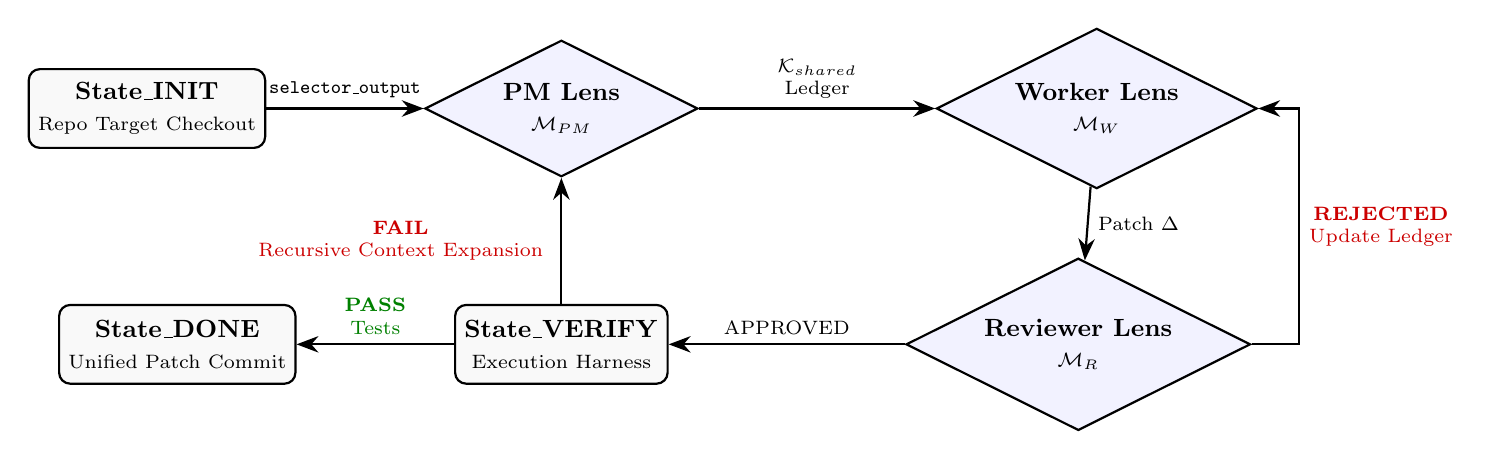
\begin{tikzpicture}[
    node distance=1.5cm and 2.0cm,
    every node/.style={font=\small, align=center},
    state/.style={draw, rectangle, minimum width=2.6cm, minimum height=1.0cm, rounded corners=4pt, thick, fill=gray!5},
    lens/.style={draw, diamond, minimum width=2.4cm, minimum height=1.0cm, aspect=2, thick, fill=blue!5},
    arrow/.style={-{Stealth[scale=1.2]}, thick}
]
    \node (init) [state] {\textbf{State\_INIT}\\\scriptsize Repo Target Checkout};
    \node (pm) [lens, right=of init] {\textbf{PM Lens}\\\scriptsize $\mathcal{M}_{\text{PM}}$};
    \node (worker) [lens, right=of pm, xshift=1.0cm] {\textbf{Worker Lens}\\\scriptsize $\mathcal{M}_{\text{W}}$};
    \node (verify) [state, below=of pm, yshift=-0.1cm] {\textbf{State\_VERIFY}\\\scriptsize Execution Harness};
    \node (reviewer) [lens, right=of verify, xshift=1.0cm] {\textbf{Reviewer Lens}\\\scriptsize $\mathcal{M}_{\text{R}}$};
    \node (done) [state, left=of verify] {\textbf{State\_DONE}\\\scriptsize Unified Patch Commit};

    \draw [arrow] (init) -- node[above, font=\scriptsize] {\texttt{selector\_output}} (pm);
    \draw [arrow] (pm) -- node[above, font=\scriptsize] {$\mathcal{K}_{\text{shared}}$\\\scriptsize Ledger} (worker);
    \draw [arrow] (worker) -- node[right, font=\scriptsize] {Patch $\Delta$} (reviewer);

    \draw [arrow] (reviewer.east) -- ++(0.6,0) |- node[pos=0.25, right, font=\scriptsize, color=red!80!black] {\textbf{REJECTED}\\Update Ledger} (worker.east);
    \draw [arrow] (reviewer) -- node[above, font=\scriptsize] {APPROVED} (verify);
    \draw [arrow] (verify) -- node[above, font=\scriptsize, color=green!50!black] {\textbf{PASS}\\Tests} (done);
    \draw [arrow] (verify.north) -- node[left, font=\scriptsize, color=red!80!black, xshift=-0.1cm] {\textbf{FAIL}\\Recursive Context Expansion} (pm.south);
\end{tikzpicture}%
}
\caption{The Context Sphere orchestration state machine. Static structural rejections continuously refine the local constraint ledger, while functional test-suite failures trigger mid-trajectory neighborhood expansion.}
\Description{State-machine diagram showing State INIT flowing through PM, Worker, Reviewer, Verify, and Done states, with rejection looping back to Worker and verification failure looping back for recursive context expansion.}
\label{fig:state_machine}
\end{figure*}

To illustrate the breakdown of traditional codebase manipulation pipelines, consider the architectural regression instance \texttt{wagtail\_\_wagtail-1120} from the SWE-bench validation suite. The issue requires refactoring notification logic inside an administrative subsystem, removing an implicit asynchronous Celery execution pathway and converting the relevant email notification behavior toward direct Django execution.

\subsection{The Failure of Static Retrieval}

A snippet-based dense retrieval pipeline queries the repository using vectors derived from the natural-language issue description. In the successful part of the run, the selector can identify the administrative file handling notification dispatches as a likely locus of the bug. However, static source splitters often chunk files according to line ranges or character limits rather than dependency semantics. The retrieved payload may therefore contain the core body functions while omitting conditional imports, environment checks, decorators, or module-level compatibility code positioned elsewhere in the file.

This partial view leaves the Worker in an informational vacuum. A single-turn LLM may generate a locally plausible synchronous replacement that appears valid within the retrieved block, yet fails to account for adjacent execution contracts defined outside the snippet. The failure is not purely semantic retrieval error; it is a structural representation error. The retrieval unit is too flat to preserve the program neighborhood around the change.

\subsection{The Multi-Agent Sycophancy Trap}

An opposite strategy passes broad source context into an extended prompt and asks collaborating agents to debate the fix. This improves coverage, but it can produce a different failure mode. If a reviewer persona consumes the same diluted prompt as the worker, lacks an explicit contract ledger, and is asked for open-ended feedback, it may default to surface-level confirmation. The resulting review appears collaborative while missing silent logic errors, missing imports, or configuration mismatches.

The Context Sphere addresses these vulnerabilities in two ways. First, it expands the centroid file through AST-derived local dependencies before prompting, grounding generation in a bounded architectural neighborhood. Second, it formalizes multi-persona interaction as a state machine over a persistent JSON constraint ledger. The Reviewer is not merely invited to comment; it must emit an explicit \texttt{APPROVED} or \texttt{REJECTED} state. Rejections are serialized into the next Worker turn, turning critique into state rather than leaving it as conversational residue.

\subsection{Observed Convergence Signal}

In the live \texttt{wagtail\_\_wagtail-1120} trace, the Worker required three attempts before internal approval. The first two attempts were rejected by the Reviewer for structural contract failures, and the rejection diagnostics were folded into the active constraints before the next generation turn. This trace does not by itself prove that the final patch is benchmark-correct. It does, however, demonstrate the intended operational behavior: reviewer critique can alter the subsequent patch search path instead of collapsing into immediate approval.

\begin{figure}[!b]
\centering
\resizebox{\columnwidth}{!}{%
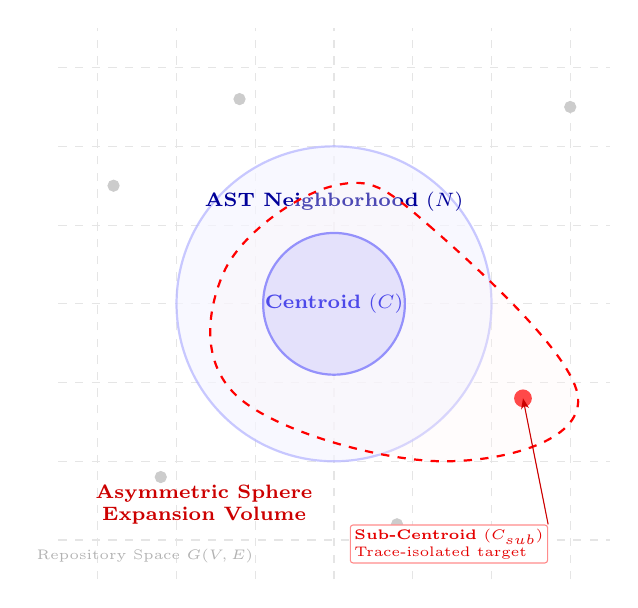
\begin{tikzpicture}
    \draw[dashed, color=gray!20] (-3.5,-3.5) grid (3.5,3.5);

    \begin{scope}
        \draw[fill=blue!4, draw=blue!30, thick, opacity=0.7] (0,0) circle (2.0cm);
        \draw[fill=blue!15, draw=blue!60, thick] (0,0) circle (0.9cm);
    \end{scope}

    \node[color=blue!90!black, font=\scriptsize] at (0,0) {\textbf{Centroid} ($C$)};
    \node[color=blue!60!black, font=\scriptsize] at (0,1.3) {\textbf{AST Neighborhood} ($N$)};

    \foreach \p in {(-2.8,1.5), (-2.2,-2.2), (3.0,2.5), (0.8,-2.8), (-1.2,2.6)}
        \filldraw[color=gray!40] \p circle (2pt);

    \coordinate (subcentroid) at (2.4,-1.2);
    \filldraw[color=red] (subcentroid) circle (3pt);

    \draw[red, dashed, thick, fill=red!4, fill opacity=0.3]
        plot[smooth cycle, tension=0.65]
        coordinates {(0,1.5) (1.2,1.0) (3.1,-1.2) (1.4,-2.0) (-1.2,-1.2) (-1.4,0.4)};

    \node[color=red!80!black, font=\scriptsize, align=center] at (-1.65,-2.55)
        {\textbf{Asymmetric Sphere}\\\textbf{Expansion Volume}};

    \node[draw=red!45, fill=white, rounded corners=1pt, inner sep=1.5pt,
          text=red!90!black, font=\tiny, align=left, anchor=west]
          (subLabel) at (0.2,-3.05)
          {\textbf{Sub-Centroid} ($C_{\text{sub}}$)\\Trace-isolated target};
    \draw[-{Stealth[scale=0.8]}, thin, color=red!80!black] (subLabel.north east) -- (subcentroid);

    \node[color=gray!60, font=\tiny] at (-2.4,-3.2) {Repository Space $G(V,E)$};
\end{tikzpicture}%
}
\caption{Geometric conceptualization of dynamic context expansion. Following a verification error, the sphere mutates from a symmetric one-hop volume to an asymmetric topological field absorbing the explicit failure-trace coordinates.}
\Description{Diagram of a code repository as a graph-like space with an initial centroid, a surrounding AST neighborhood, and an asymmetric red expansion toward a trace-isolated sub-centroid.}
\label{fig:spatial_sphere}
\end{figure}

\section{Related Work}
\label{sec:related_work}

Our framework interfaces with three paradigms in software automation: automated program repair, code-centric retrieval, and collaborative multi-agent system design.

\subsection{Automated Program Repair}

Traditional automated program repair (APR) systems rely on search-based heuristics, genetic programming, templates, or semantic constraints to manipulate programs under a test or specification signal. These methods can provide strong precision within localized settings, but often depend on concrete test suites or other executable specifications~\cite{legoues2019apr}. SWE-bench reframed this challenge for language-model agents by evaluating whether a model can edit real repositories in response to natural-language issues~\cite{jimenez2024swebench}. The Context Sphere builds on this problem setting, but focuses on the context-orchestration layer: how an agent should select, expand, and reuse repository evidence before and during patch generation.

\subsection{Repository Retrieval Pipelines}

Codebase retrieval systems commonly map natural-language issues to files, functions, or chunks using lexical retrieval, embeddings, reranking, or learned selectors. This makes large repositories tractable, but standard retrieval can ignore the dependency topology that makes a code edit valid. RepoCoder demonstrates an iterative retrieval-generation loop for repository-level code completion, while long-context studies show that adding more context is not always sufficient because models can fail to use information buried in the middle of a prompt~\cite{zhang2023repocoder,liu2024lost}. Graph-structured code models and graph-based repository retrieval methods further motivate topology-aware context, but they often require richer graph construction or graph-aware representation learning~\cite{guo2021graphcodebert,liu2024graphcoder}. The Context Sphere occupies a narrower and more lightweight point in this design space: a neural selector identifies the likely issue centroid, and a deterministic AST expansion step restores immediate local dependencies.

\subsection{Multi-Persona LLM Architectures}

Multi-agent software systems such as ChatDev, MetaGPT, and SWE-agent demonstrate that LLMs can be organized into role-specific workflows for design, coding, testing, repository navigation, and tool use~\cite{qian2024chatdev,hong2024metagpt,yang2024sweagent}. These systems motivate role separation, but open-ended dialogue can accumulate prompt noise and confirmation bias. Sycophancy studies show that assistant models can prefer responses that align with user beliefs over truthful correction, motivating stricter reviewer boundaries~\cite{sharma2023sycophancy}. The Context Sphere differs by coupling role separation to a bounded repository neighborhood and by forcing Worker--Reviewer iteration through a structured constraint ledger.

\subsection{Cost-Aware Agent Deployment}

End-to-end coding agents are increasingly evaluated as systems rather than isolated generation calls. This motivates cost-aware reporting alongside correctness, since long-horizon repository repair can require many retrieval, editing, review, and verification turns. HAL and SWE-Effi both reflect this shift by surfacing resource consumption together with task performance~\cite{princetonhal2026,fan2025sweeffi}. Our work follows this direction by reporting local repair success together with token and cost estimates, and by treating context selection as an optimization target rather than an implementation detail.

\subsection{LLM-as-Judge Reliability}

Although the primary ablation reports execution-checked outcomes under a local harness, LLM-as-judge reliability remains relevant because the orchestration loop still uses a Reviewer persona before verification. Prior work on LLM-based judging has documented position, verbosity, and self-enhancement biases~\cite{zheng2023judging}. Accordingly, this paper treats internal approval as an intermediate control signal. Official benchmark execution, gold-patch comparison, and swapped-order judging remain necessary before claiming leaderboard-level repair correctness.

\section{The Context Sphere Architecture}
\label{sec:approach}

The conceptual foundation of the framework is a spatial representation of software repositories. We model a repository as a directed dependency graph \(G=(V,E)\), where \(V=\{f_1,f_2,\dots,f_n\}\) represents source files or partitioned code chunks, and \(E=\{(f_i,f_j)\}\) represents explicit program dependencies such as module imports, local definitions, or configuration requirements.

\subsection{Formalizing the Spatial Volume}

The construction of an issue-specific Context Sphere proceeds through a dual-layer neural and deterministic pipeline:

\begin{enumerate}
    \item \textbf{Centroid isolation (\(C\)):} Given an unstructured issue specification \(I\), the Locator scores repository blocks and extracts the top-ranked modules or chunks to instantiate the problem's core centroid set:
    \begin{equation}
        C = \{v \in V \mid \text{Score}(v, I) > \tau\},
    \end{equation}
    where \(\tau\) represents a configured retrieval activation threshold.

    \item \textbf{Neighborhood expansion (\(N\)):} To prevent structural data loss caused by static chunk boundaries, the Assembler executes a local one-hop dependency sweep from the centroid coordinates. An AST crawler parses files within \(C\), extracts internal import paths, and builds the neighborhood set:
    \begin{equation}
        N(C) = \{u \in V \mid \exists v \in C \text{ s.t. } (v,u) \in E\}.
    \end{equation}

    \item \textbf{Unified sphere aggregation (\(S\)):} The bounded context space passed to the orchestration pipeline is the union of the centroid and its local neighborhood:
    \begin{equation}
        S = C \cup N(C).
    \end{equation}
\end{enumerate}

\subsection{Persona Projection and Context Lenses}

Rather than processing \(S\) through a single monolithic prompt, the framework projects the same bounded volume into three decoupled persona lenses:

\begin{itemize}
    \item \textbf{Product Manager lens (\(\mathcal{M}_{\text{PM}}\)):} Projects the issue and spatial volume \(S\) into explicit acceptance criteria and risk constraints, producing a persistent validation contract \(\mathcal{K}_{\text{shared}}\) stored as \texttt{constraints.json}.
    \item \textbf{Worker lens (\(\mathcal{M}_{\text{W}}\)):} Consumes \(S \cup \mathcal{K}_{\text{shared}}\) and operates on implementation mechanics, control flow, imports, and local test expectations, outputting a candidate patch delta \(\Delta\).
    \item \textbf{Reviewer lens (\(\mathcal{M}_{\text{R}}\)):} Evaluates \(\Delta\) against the bounded neighborhood \(S\), blocking structural regressions and returning a verification state \(\mathcal{V} \in \{\texttt{APPROVED}, \texttt{REJECTED}\}\).
\end{itemize}

\subsection{Stateful Adversarial Feedback Loop}

The orchestrator manages a correction task as a deterministic state machine:
\[
\texttt{INIT} \rightarrow \texttt{PM} \rightarrow \texttt{WORKER}
\rightarrow \texttt{REVIEWER}.
\]
If the Reviewer returns \(\mathcal{V}=\texttt{REJECTED}\), the orchestrator serializes the reviewer's diagnostics into \(\mathcal{K}_{\text{shared}}\) and routes execution back to the Worker. The loop continues until either the Reviewer returns \(\mathcal{V}=\texttt{APPROVED}\) or a fixed attempt budget is exhausted, at which point the run terminates with manual intervention.

This design turns review into a state transition rather than a conversational suggestion. The Worker cannot simply ignore a prior critique, because the critique becomes part of the shared constraint ledger consumed on the next turn. The Reviewer, similarly, must choose between explicit approval and explicit rejection, giving the evaluation trace a measurable convergence structure.

\section{System Implementation Details}
\label{sec:implementation}

The production architecture of the Context Sphere framework is partitioned into three decoupled programmatic modules: the neural Locator (\path{inference.py}), the topology-aware Assembler (\path{assembler.py}), and the stateful Orchestrator (\path{orchestrate_resolution.py}). This section describes the runtime configuration and engineering boundaries for each module.

\subsection{The Locator: Neural Selection Field}

The pipeline starts from raw, unstructured issue text. The issue description is passed to the trained selector, which scores visible issue chunks and candidate repository files for language-to-code relevance. The codebase under review is partitioned into bounded code blocks or function-level text segments:

\begin{equation}
    B = \{b_1, b_2, \dots, b_m\} \subseteq V .
\end{equation}

The selector computes an alignment score representing whether a block or file is likely to contain, constrain, or directly command the root cause of the regression. The top-\(K\) highest-scoring blocks and projected files establish the initial coordinates of the problem space, acting as the Context Sphere centroid \(C\). Current selector evidence is selector-only: it measures ranking against touched-file labels and does not by itself prove patch correctness.

\subsection{Training the Context Locator}

The Context Locator is trained as a neural file-relevance model: given a visible issue description and candidate repository file content, it predicts whether the file belongs in the initial centroid set. Training examples are derived from SWE-bench training instances using touched-file supervision, with validation grouped by \textit{case\_slug} so that files from the same issue instance do not appear in both train and validation splits.

The Locator uses a MiniLM-family cross-encoder backbone and is optimized with binary cross-entropy over issue--file pairs. Gold-patch contents are not exposed as model input: patch-derived information is used only to construct touched-file labels, while the visible training features consist of issue text, file paths, and repository source content available before solving the task. This leakage boundary is important because the Locator should learn structural relevance, not memorize solution diffs. The trained Locator produces the relevance scores consumed by the Assembler, making it the learned entry point for Context Sphere construction.

\subsection{The Assembler: AST Neighborhood Expansion}

Once the centroid coordinates are fixed, the Assembler performs a deterministic local Abstract Syntax Tree (AST) crawl to reconstruct nearby program dependencies. This prevents the information amputation that often occurs when vector retrieval returns an isolated snippet without its imported helpers or adjacent contracts.

\begin{itemize}
    \item \textbf{Import subgraph parsing:} The assembler reads each centroid file and builds a local syntax tree using Python's native \path{ast} parser. It extracts \path{Import} and \path{ImportFrom} declarations.
    \item \textbf{Local module resolution:} Extracted import paths are matched against the repository root. If a matching internal module is verified, its source text is appended to the Neighborhood set \(N\).
    \item \textbf{Context window clamping:} To bound context size and preserve attention density, file content is clipped by a character threshold \(L_{\max}\), exposed through the \path{--max-file-chars} flag:
    \begin{equation}
        S_{\text{bounded}} = \{f \in S \mid \mathrm{Length}(f) \le L_{\max}\}.
    \end{equation}
\end{itemize}

The current assembler is intentionally conservative: it resolves one-hop Python imports under local repository paths and ignores unresolved, standard-library, or cross-language imports rather than guessing.

\subsection{The Orchestrator: Multi-Persona State Machine}

Runtime coordination is handled by a stateful sequence orchestrator that manages prompt construction, model calls, reviewer feedback, and artifact persistence. The state transitions proceed through:

\begin{enumerate}
    \item \textbf{\path{State_INIT}:} Ingests the \path{selector_output.json} coordinates file, checks out the target repository to its base Git commit, and initializes the run directory.
    \item \textbf{\path{State_PM}:} Projects the context sphere through a planning lens and writes a structured persistent constraint ledger, \path{constraints.json}.
    \item \textbf{\path{State_WORKER}:} Bundles core evidence, neighborhood modules, and the live constraint ledger into an implementation prompt. The Worker persona generates a unified patch candidate \(\Delta\).
    \item \textbf{\path{State_REVIEWER}:} Evaluates \(\Delta\) against the context graph. The Reviewer returns either \path{APPROVED} or \path{REJECTED}. Rejection appends diagnostic critique back into the live ledger and triggers the next Worker attempt.
\end{enumerate}

The result is not an unstructured chat among agents. It is a bounded state machine with persistent artifacts: selector output, persona-specific spheres, PM constraints, per-attempt patches, reviewer reports, final patch candidates, and manual-intervention records.

\subsection{Fault-Tolerant Dynamic Provider Fallback}

Production-scale repository repair runs are exposed to API volatility. Multi-turn Context Sphere trajectories can encounter rate limits, quota exhaustion, transient server failures, or gateway timeouts before the state machine reaches a terminal state. A provider failure at this layer should not erase the already-constructed context sphere, constraint ledger, or reviewer feedback history.

The orchestrator therefore supports a fallback routing profile that separates persona state from backend provider state. Under this profile, persona calls are attempted first through the primary DeepSeek \texttt{deepseek-chat} route. If the primary route raises a fallbackable provider error, including HTTP 429, quota-like failures, timeout errors, or HTTP 5xx gateway/server failures, the runtime records a provider-swap event and retries the same uncompressed prompt payload through a secondary MiniMax-compatible chat-completions backend. The retry preserves the current PM, Worker, or Reviewer state and does not rebuild the surrounding run directory.

Provider swaps are written into the run summary as structured metadata, including the role, attempt index, source provider/model, destination provider/model, sanitized error detail, and timestamp. Token and cost accounting are attributed to the backend that actually produced the response, so a mid-run swap changes subsequent usage totals without corrupting the global \path{model_usage} ledger. This design makes provider continuity an execution concern rather than a cognitive concern: the agent personas continue from the same state machine boundary while the backend abstraction absorbs transient provider failure.

\section{Research Questions}

\textbf{RQ1: Role sufficiency.} Do planner, worker, and reviewer agents require measurably different context bundles?

\textbf{RQ2: Reviewer behavior.} Under controlled evidence visibility, do role-conditioned contexts improve critical-issue recall, evidence grounding, or independence from author framing?

\textbf{RQ3: Selector quality.} Can role-conditioned retrieval recover task-relevant files or chunks with fewer tokens than full context and standard retrieval baselines?

\textbf{RQ4: End-to-end utility.} When paired with an LLM generator and evaluated through an execution harness, does role-conditioned context allocation preserve or improve task success under lower context cost?

The current 100-case ablation provides local \texttt{PASS\_TO\_PASS} evidence for RQ4; official SWE-bench \texttt{FAIL\_TO\_PASS} scoring remains a stricter follow-up target.

\section{Methodology}

\subsection{Task Selection}

The primary evaluation uses 100 pure-Python instances sampled from SWE-bench Verified. The sample emphasizes repositories whose dependency structure can be handled by the current Python AST Assembler: \texttt{django/django}, \texttt{sphinx-doc/sphinx}, \texttt{psf/requests}, \texttt{pytest-dev/pytest}, and \texttt{pallets/flask}. Each instance is initialized at the benchmark base commit and paired with the issue text used to construct the retrieval query.

The Locator selector was trained with patch-level supervision from a separate training subset. During evaluation, retrieval uses only the issue text and repository snapshot available at the base commit; gold-patch content is strictly excluded from inference-time retrieval to maintain an adversarial setting.

\subsection{Retrieval Configurations}

We compare three retrieval configurations under the same downstream PM--Worker--Reviewer orchestration protocol:
\begin{itemize}
    \item \textbf{Dense Vector baseline:} ranks repository files using dense semantic similarity between the issue text and file contents.
    \item \textbf{Context Sphere:} identifies a centroid using the Locator and then expands the context through one-hop AST-derived local dependencies.
    \item \textbf{Hybrid:} merges dense Vector and Context Sphere candidates using a dense-first ordering policy.
\end{itemize}
Holding the generator, reviewer, verification harness, and attempt budget fixed isolates the retrieval policy as the controlled variable.

All three retrieval configurations used the same retrieval and repair budget: top-\(K=5\) core files, a maximum of 24 one-hop neighborhood files, a maximum file-character clamp of 60{,}000 characters, and at most three Worker--Reviewer repair attempts per issue.

\subsection{Model and Provider Configuration}

Unless otherwise stated, PM, Worker, and Reviewer calls in the 100-case ablation used the fallback routing profile with DeepSeek \texttt{deepseek-chat} as the primary OpenAI-compatible backend and MiniMax \texttt{MiniMax-M2.7} as the secondary backend. Locator and Assembler stages were local scripts and did not invoke completion models. Provider fallback was enabled only when primary calls failed due to rate limits, quota or payment errors, timeouts, or server-side errors. Token and cost accounting were attributed to the backend that produced each response.

\subsection{Verification Signal}

For each run, the orchestrator emits a candidate patch, applies it to the checked-out repository, and executes the configured local regression command. We count a local pass only when the patch applies cleanly and the command exits successfully. This is a local \texttt{PASS\_TO\_PASS} smoke/regression signal. It is stricter than internal reviewer approval, but it is not equivalent to official SWE-bench \texttt{FAIL\_TO\_PASS} scoring because the hidden benchmark test patch is not applied.

\subsection{Metrics}

The primary metric is local \texttt{PASS\_TO\_PASS} pass count across the 100 intended cases. Secondary metrics include pass overlap across retrieval methods, patch-application failure buckets, total model invocations, and estimated inference cost. Cost is computed from provider-specific token coefficients and emitted per case in the metrics ledger. We report relative improvement over the dense Vector baseline as:
\[
    \frac{\text{Passes}_{\text{Context Sphere}} - \text{Passes}_{\text{Vector}}}
    {\text{Passes}_{\text{Vector}}}.
\]

\subsection{Reproducibility Artifacts}

The paper results are grounded in the local comparative report generated from \path{outputs/ablation_100_vector}, \path{outputs/ablation_100_context}, and \path{outputs/ablation_100_hybrid}. The report reconstructs aggregate statistics from per-case metrics because one case terminated before aggregate summary writing. We therefore treat the crashed case as a non-pass for all methods.

\subsection{Projection Smoke Cohort}

The Context Projection Model is evaluated as a follow-on smoke test over the first 10 cases that passed under the 100-case Context Sphere run. This design intentionally measures whether persona-conditioned projection can preserve known successes while reducing context load. It should not be interpreted as an unbiased repair benchmark. The projection comparison is generated from \path{outputs/projection_smoke_10_fallback} and \path{outputs/projection_smoke_10_floor}.

\section{Empirical Evaluation}
\label{sec:evaluation}

We evaluated Context Sphere with a 100-case retrieval ablation over pure-Python instances sampled from SWE-bench Verified. The ablation compares three retrieval configurations while holding the downstream orchestration and verification harness fixed: a dense Vector baseline, Context Sphere retrieval, and a Hybrid configuration that concatenates dense-vector and Context Sphere candidates.

\subsection{Benchmark Composition}

The benchmark contains 100 pure-Python issue instances sampled from stable SWE-bench Verified repositories. The distribution is dominated by \texttt{django/django} and \texttt{sphinx-doc/sphinx}, with additional cases from \texttt{psf/requests}, \texttt{pytest-dev/pytest}, and \texttt{pallets/flask}. This slice was selected to stress repository-local dependency mapping while avoiding polyglot parser confounds.

One generated test command produced a runner crash before the aggregate summary writer completed, so the local artifact set contains 99 written metric records for each retrieval method. We conservatively count the crashed instance as a non-pass for all methods and report results over the intended 100-case benchmark. The verification signal is the local \texttt{PASS\_TO\_PASS} smoke/regression harness, not official SWE-bench \texttt{FAIL\_TO\_PASS} scoring.

\subsection{Resource-Constrained Optimization Framework}

Recent agent evaluation frameworks increasingly report task outcomes together with resource consumption. The Holistic Agent Leaderboard (HAL) explicitly incorporates cost-controlled evaluation and token trace tracking~\cite{princetonhal2026}, while SWE-Effi argues that software-agent systems should be ranked by both issue-resolution outcomes and resources such as tokens and time~\cite{fan2025sweeffi}. We therefore record inference cost as a first-class metric rather than treating completion rate in isolation.

\subsubsection{System Inference Cost}
Let \(\mathcal{T}=\{1,2,\dots,T\}\) denote the sequential execution path for one issue-resolution run. At each turn \(t \in \mathcal{T}\), the active persona invokes model \(\mathcal{M}_t\). We define estimated system inference cost as:
\begin{equation}
    C_{\mathrm{sys}} = \sum_{t=1}^{T}
    \left(
        \phi_{\mathrm{in}}(\mathcal{M}_t) X_{\mathrm{in}}(t)
        + \phi_{\mathrm{out}}(\mathcal{M}_t) X_{\mathrm{out}}(t)
    \right),
\end{equation}
where \(X_{\mathrm{in}}(t)\) and \(X_{\mathrm{out}}(t)\) are input and output token counts for turn \(t\), and \(\phi_{\mathrm{in}}\) and \(\phi_{\mathrm{out}}\) are per-token cost coefficients for the selected deployment profile.

\subsubsection{Efficacy per Dollar}
For verification-enabled runs, we define a binary success indicator \(R_{\mathrm{verify}}\in\{0,1\}\), where \(R_{\mathrm{verify}}=1\) only when the final candidate patch applies cleanly and passes the configured repository regression command. The efficacy-per-dollar coefficient is:
\begin{equation}
    \eta_{\mathrm{cost}} = \frac{R_{\mathrm{verify}}}{C_{\mathrm{sys}}}.
\end{equation}
The cohort-level value \(\bar{\eta}_{\mathrm{cost}}\) exposes the Pareto trade-off between repair success and infrastructure expense.

We use this formulation primarily for per-run accounting and artifact-level comparison; the present paper reports aggregate cost and pass counts rather than ranking systems solely by \(\bar{\eta}_{\mathrm{cost}}\).

\subsection{100-Case Retrieval Ablation}

Table~\ref{tab:verified-ablation-100} summarizes the completed ablation. Context Sphere achieved 41 successful local repair passes, compared with 36 passes for the dense Vector baseline and 39 passes for the Hybrid configuration. This corresponds to an approximately 13.8\% relative improvement over the dense Vector baseline:
\begin{equation}
    \frac{41 - 36}{36} \times 100 \approx 13.8\%.
\end{equation}

\begin{table}[t]
\centering
\caption{100-case SWE-bench Verified retrieval ablation under the local \texttt{PASS\_TO\_PASS} verification harness.}
\label{tab:verified-ablation-100}
\resizebox{\columnwidth}{!}{%
\begin{tabular}{lccc}
\toprule
\textbf{Retrieval Configuration} & \textbf{Local \texttt{PASS\_TO\_PASS} Passes} & \textbf{Pass Rate} & \textbf{Relative to Vector} \\
\midrule
Dense Vector baseline & 36 / 100 & 36.0\% & -- \\
Context Sphere & \textbf{41 / 100} & \textbf{41.0\%} & \textbf{+13.8\%} \\
Hybrid & 39 / 100 & 39.0\% & +8.3\% \\
\bottomrule
\end{tabular}%
}
\end{table}

Within this benchmark slice, Context Sphere produced the highest local pass count among the three retrieval architectures. The result is consistent with the central hypothesis that deterministic structural dependency mapping supplies repair-relevant context that dense lexical or semantic retrieval can miss.

\subsection{Cost and Failure Profile}

The Context Sphere run recorded an estimated aggregate inference spend of \(\$8.202211\) across the 100-case campaign. In this local configuration, the framework operated at approximately \$0.08 per issue, suggesting that topology-aware context selection may be useful for cost-sensitive repository-repair pipelines.

The dominant shared bottleneck across all three retrieval methods was not model invocation volume but patch materialization. Patch-application failures accounted for 31 Vector failures, 27 Context Sphere failures, and 24 Hybrid failures. This indicates that future gains require improving both retrieval routing and the patch application layer: better context alone cannot recover patches that cannot be applied to the target checkout.

\subsection{Prior Pilot Traces}

Before the 100-case ablation, the system was evaluated on a smaller 15-case live orchestrator slice. That pilot measured internal reviewer approval rather than execution-verified patch success and reached 7/15 internal approvals. We treat those traces as mechanism evidence for the adversarial feedback loop, not as the primary empirical result of the paper.

\section{Discussion}
\label{sec:discussion}

\subsection{Internal Approval Versus Correctness}

The most important interpretive boundary is that our early live traces measured internal reviewer approval, while the 100-case ablation measures local execution-verified \texttt{PASS\_TO\_PASS} outcomes. The latter is a stronger signal, but it is still not identical to official SWE-bench \texttt{FAIL\_TO\_PASS} scoring. We therefore treat the ablation as evidence about retrieval architecture under a fixed local verification harness, not as a final leaderboard claim.

\subsection{The Hybrid Paradox}

The ablation produced a counterintuitive result: Hybrid retrieval achieved 39 successful local repair passes, slightly underperforming the Context Sphere configuration at 41 passes. The pass-overlap matrix shows a 51/100 theoretical ceiling, meaning at least one retrieval method solved 51 distinct issues. This suggests that the underlying orchestration agent can solve more cases than any single retrieval policy currently exposes.

The likely cause is the \textit{Dense-First Merge Policy}. In the Hybrid configuration, high-scoring lexical or semantic matches from the dense Vector retriever were placed before structurally selected dependency files. On some cases, these dense matches acted as context noise and displaced the local dependency files that Context Sphere alone would have supplied. The result is not a rejection of hybrid retrieval; it is evidence that naive concatenation is a weak routing policy. Future retrieval systems should use score-normalized interleaving or learned routing to balance lexical relevance against structural dependency evidence.

The same analysis exposes a shared engineering bottleneck. Patch application remained the primary cross-method failure mode, with dozens of failures across all retrieval configurations. Retrieval improvements must therefore be paired with stronger patch materialization and checkout-aware edit application.

\subsection{Research Interpretation}

The strongest current claim is not that Context Sphere solves autonomous bug resolution. The defensible claim is that topology-aware neighborhood expansion improves verified outcomes over a dense Vector baseline on this 100-case pure-Python slice, while the remaining 51-case overlap ceiling and patch-application failures identify where retrieval routing, neighborhood expansion, and edit materialization still break.

\section{Preliminary Investigation: Token-Efficient Projection Routing}
\label{sec:projection}

The 100-case ablation shows that retrieval policy, not only model capability, determines whether the orchestrator receives useful evidence. To optimize this bottleneck, we implemented a Context Projection Model trained as a persona-conditioned cross-encoder. The projector operates after Master Context Sphere assembly and before persona prompting, scoring candidate graph nodes separately for the Product Manager, Worker, and Reviewer.

\subsection{Training Methodology}

The projection model was trained on 7{,}299 training samples with an 888-row held-out validation split. Training used the \texttt{cross-encoder/ms-marco-MiniLM-L-6-v2} backbone on Apple Silicon MPS. To address the severe class imbalance in implementation-level routing, we applied persona-stratified oversampling, increasing Worker-positive training rows from 109 to 279 while preserving the grouped validation split. The model was optimized with asymmetric binary cross-entropy using persona-specific positive weights (Worker=18, Reviewer=10, PM=8) and a negative weight of 1.0.

We selected the final checkpoint using a Worker Margin criterion, defined as the validation mean score for Worker-positive rows minus the validation mean score for Worker-negative rows. This early-stopping rule selected the Epoch 1 checkpoint, before later optimization could overfit easier PM/Reviewer structural labels and degrade the fragile Worker routing signal. The released artifact repository includes the training scripts, saved report, thresholds, validation scores, and model checkpoint metadata.

\subsection{Asymmetric Cognitive Routing}

The projection task is asymmetric across personas. Product Manager and Reviewer prompts benefit from high-precision structural skeletons: paths, interfaces, tests, imports, and risk-bearing adjacency. Worker prompts require higher-recall code access because implementation often depends on local function bodies and nearby edit anchors. Initial training exposed gradient starvation for implementation-level routing, where Worker-positive evidence was underrepresented relative to easier structural negatives.

\subsection{Safety Floors Against Context Starvation}

Aggressive thresholding reduced token load but created a failure mode we call \textit{context starvation}: a persona could receive too few nodes to maintain a coherent local view. In the no-floor projection smoke test, the Reviewer often received zero selected nodes, and the pass rate dropped to 6/10 on a cohort that full Context Sphere solved completely. We therefore added a deterministic Top-\(K\) safety floor with \(min\_k=2\), ensuring that every persona receives at least two context anchors even when calibrated model confidence is low.

\subsection{Projection Smoke Results}

Table~\ref{tab:projection_results} summarizes the projection smoke test. The cohort consists of 10 cases selected from Context Sphere successes in the 100-case ablation, so the baseline pass rate is intentionally 10/10. With the Top-\(K\) safety floor, projection preserved 9/10 passes while reducing input tokens by 71.5\% and estimated inference cost by 58.4\%.

\begin{table}[t]
\centering
\caption{Projection-mode routing on a 10-case Context Sphere success cohort.}
\label{tab:projection_results}
\resizebox{\columnwidth}{!}{%
\begin{tabular}{lccc}
\toprule
\textbf{Metric} & \textbf{Full Context Sphere} & \textbf{Projection (\(min\_k=2\))} & \textbf{Change} \\
\midrule
Local pass rate & 10 / 10 & 9 / 10 & -10.0\% \\
Total tokens & 2{,}090{,}215 & 643{,}512 & \textbf{-69.2\%} \\
Input tokens & 2{,}078{,}983 & 592{,}935 & \textbf{-71.5\%} \\
Context characters & 8{,}483{,}908 & 1{,}979{,}745 & \textbf{-76.7\%} \\
Inference cost & \$0.5737 & \$0.2386 & \textbf{-58.4\%} \\
\bottomrule
\end{tabular}%
}
\end{table}

This result reframes projection as a resource-control layer rather than a replacement for the Context Sphere. The Master Sphere remains responsible for broad structural recall; projection converts that master topology into persona-specific Spheres of Influence that constrain token load while preserving enough evidence for downstream repair.

\section{Limitations}
\label{sec:limitations}

Our study is subject to several limitations that we aim to address in future iterations.

\textbf{Evaluation protocol.} Metrics are derived from a local \texttt{PASS\_TO\_PASS} regression harness rather than the official SWE-bench Verified evaluation protocol. The results therefore characterize retrieval behavior under our local verifier and should not be interpreted as official leaderboard scores.

\textbf{Selector supervision and leakage risk.} The Locator selector was trained using patch-label supervision. Although evaluation excludes gold-patch content during retrieval, issue metadata can still leak correlations from historical tasks. A stronger protocol should include time-split tasks, less-public repositories, and explicit model-version provenance.

\textbf{Projection scope.} The Context Projection Model results are derived from a preliminary 10-case smoke test selected from known Context Sphere successes. These results demonstrate routing efficiency and context-starvation mitigation, but they are not a comprehensive projection benchmark.

\textbf{Projection training leakage protection.} The projection dataset is constructed from retrieved node features and persona labels derived from training-split instances. Gold-patch solution code is excluded from the projection feature set, and the projection model is trained to route candidate context nodes rather than to predict patch text. Nevertheless, because the broader benchmark uses public repositories and public issue metadata, future work should repeat the training protocol on time-split or private repositories.

\textbf{Architectural scope.} The current implementation focuses on pure-Python repositories to enable reliable AST-based dependency resolution. The current Assembler resolves one-hop Python imports; this boundary keeps the context window compact, but it can miss deep inheritance chains, plugin registries, dynamic imports, and polyglot repository flows. Extending Context Sphere to TypeScript, Go, Java, C++, and mixed enterprise systems will require broader parser and import-resolution layers.

\textbf{Patch materialization.} Patch application remained the dominant shared failure mode across retrieval configurations. Future work must pair retrieval improvements with checkout-aware edit materialization, stronger patch parsers, and stricter execution feedback.

\section{Reproducibility and Artifacts}
\label{sec:reproducibility}

All experiments were conducted using the local verification harness described in Sec.~\ref{sec:evaluation}. Results are reconstructed from per-case metrics stored under:
\begin{itemize}
    \item \path{outputs/ablation_100_vector}
    \item \path{outputs/ablation_100_context}
    \item \path{outputs/ablation_100_hybrid}
    \item \path{outputs/projection_smoke_10_fallback}
    \item \path{outputs/projection_smoke_10_floor}
\end{itemize}

The full framework (Locator, AST Assembler, multi-persona Orchestrator, and Projection Model) is implemented in Python. The exact 100-case instance list is included in the artifact repository to support reproduction and paired comparison across retrieval configurations.

The artifact repository also includes the retrieval configuration files and per-case result ledgers used to reconstruct Tables~\ref{tab:verified-ablation-100},~\ref{tab:efficiency-profile}, and~\ref{tab:projection_results}. Full reproduction instructions, configuration files, case lists, result ledgers, and model metadata are available at \url{https://github.com/johnZYW/context-sphere}. The trained Context Locator and Context Projection checkpoints are released on Hugging Face at \url{https://huggingface.co/Zywdd/context-sphere-locator} and \url{https://huggingface.co/Zywdd/context-sphere-projector}, respectively.

\section{Conclusion}

This paper frames Context Sphere as a falsifiable architecture for topology-aware context allocation in software-engineering agents. In the current 100-case SWE-bench Verified ablation, Context Sphere achieved 41 local \texttt{PASS\_TO\_PASS} repair passes, compared with 36 for dense Vector retrieval and 39 for a naive Hybrid retriever, at roughly \$0.08 per issue. A follow-on projection smoke test shows that persona-conditioned routing can preserve 9/10 known Context Sphere successes while reducing input-token load by 71.5\% and estimated inference cost by 58.4\%.

The ablation also exposes the next research target. While Context Sphere provides a structured topological map of the repository, the 51-pass overlap ceiling shows that no single retrieval policy captures all solvable cases. The Context Projection Model is our first step toward that target: a trained discriminative routing layer designed to slice the Master Context Sphere into token-efficient, persona-specific \textit{Spheres of Influence} for the Product Manager, Worker, and Reviewer. The next stage is to scale this projection layer beyond the preliminary smoke cohort, pair it with stronger patch materialization, and evaluate the full stack under official SWE-bench \texttt{FAIL\_TO\_PASS} conditions.

\section*{Artifact Availability}
\enlargethispage{3pt}

Code, prompts, configuration files, evaluation scripts, the 100-case instance list, result artifacts, and trained model weights are available at:

\begin{itemize}
    \item \textbf{Framework code and evaluation artifacts:} \url{https://github.com/johnZYW/context-sphere}
    \item \textbf{Context Locator weights:} \url{https://huggingface.co/Zywdd/context-sphere-locator}
    \item \textbf{Context Projection weights:} \url{https://huggingface.co/Zywdd/context-sphere-projector}
\end{itemize}

The framework repository contains instructions to reproduce the main retrieval ablation and projection experiments.


\bibliographystyle{ACM-Reference-Format}
\bibliography{main}

\end{document}
